% Taken from: https://mikedewar.wordpress.com/2009/02/25/latex-beamer-python-beauty/
\documentclass[12pt,english,pdf,xcolor=dvipsnames,aspectratio=169,handout]{beamer}\usepackage[]{graphicx}\usepackage[]{xcolor}
% maxwidth is the original width if it is less than linewidth
% otherwise use linewidth (to make sure the graphics do not exceed the margin)
\makeatletter
\def\maxwidth{ %
  \ifdim\Gin@nat@width>\linewidth
    \linewidth
  \else
    \Gin@nat@width
  \fi
}
\makeatother

\definecolor{fgcolor}{rgb}{0.345, 0.345, 0.345}
\newcommand{\hlnum}[1]{\textcolor[rgb]{0.686,0.059,0.569}{#1}}%
\newcommand{\hlstr}[1]{\textcolor[rgb]{0.192,0.494,0.8}{#1}}%
\newcommand{\hlcom}[1]{\textcolor[rgb]{0.678,0.584,0.686}{\textit{#1}}}%
\newcommand{\hlopt}[1]{\textcolor[rgb]{0,0,0}{#1}}%
\newcommand{\hlstd}[1]{\textcolor[rgb]{0.345,0.345,0.345}{#1}}%
\newcommand{\hlkwa}[1]{\textcolor[rgb]{0.161,0.373,0.58}{\textbf{#1}}}%
\newcommand{\hlkwb}[1]{\textcolor[rgb]{0.69,0.353,0.396}{#1}}%
\newcommand{\hlkwc}[1]{\textcolor[rgb]{0.333,0.667,0.333}{#1}}%
\newcommand{\hlkwd}[1]{\textcolor[rgb]{0.737,0.353,0.396}{\textbf{#1}}}%
\let\hlipl\hlkwb

\usepackage{framed}
\makeatletter
\newenvironment{kframe}{%
 \def\at@end@of@kframe{}%
 \ifinner\ifhmode%
  \def\at@end@of@kframe{\end{minipage}}%
  \begin{minipage}{\columnwidth}%
 \fi\fi%
 \def\FrameCommand##1{\hskip\@totalleftmargin \hskip-\fboxsep
 \colorbox{shadecolor}{##1}\hskip-\fboxsep
     % There is no \\@totalrightmargin, so:
     \hskip-\linewidth \hskip-\@totalleftmargin \hskip\columnwidth}%
 \MakeFramed {\advance\hsize-\width
   \@totalleftmargin\z@ \linewidth\hsize
   \@setminipage}}%
 {\par\unskip\endMakeFramed%
 \at@end@of@kframe}
\makeatother

\definecolor{shadecolor}{rgb}{.97, .97, .97}
\definecolor{messagecolor}{rgb}{0, 0, 0}
\definecolor{warningcolor}{rgb}{1, 0, 1}
\definecolor{errorcolor}{rgb}{1, 0, 0}
\newenvironment{knitrout}{}{} % an empty environment to be redefined in TeX

\usepackage{alltt}
\usepackage{etex}
\usetheme{default}
\beamertemplatenavigationsymbolsempty
\definecolor{fore}{RGB}{43,41,46}
\definecolor{back}{RGB}{255,255,255}
\definecolor{title}{RGB}{198,24,38}
\setbeamercolor{titlelike}{fg=title}
\setbeamercolor{normal text}{fg=fore,bg=back}
\usepackage{mathpazo}
\usepackage{amsmath}
\usepackage{multirow}
\renewcommand{\familydefault}{\rmdefault}
\usepackage[T1]{fontenc}
\usepackage{inputenc}
\usepackage{parskip}
\setcounter{secnumdepth}{3}
\setcounter{tocdepth}{3}
\usepackage{hyperref}
\hypersetup{pdfauthor={Constantin Manuel Bosancianu},
pdftitle={Advanced Topics in Applied Regression},
pdfsubject={Day 4: Nonlinear Regression},
pdfkeywords={Budapest, ECPR, 2017, day 4, SSMT}}
\usepackage{babel}
\usepackage{graphicx}
\usepackage{subfigure}
\usepackage{palatino}
% Defines a checkmark
\def\checkmark{\tikz\fill[scale=0.4,color=title](0,.35) -- (.25,0) -- (1,.7) -- (.25,.15) -- cycle;}
\setbeamertemplate{itemize items}{\checkmark}
% For table captions in Beamer
\usepackage[labelformat=empty]{caption}
\captionsetup[figure]{labelfont={color=fore}}
\captionsetup[table]{labelfont={color=fore}}
\usepackage{tikz, tikz-cd, animate}
\usetikzlibrary{shapes,backgrounds,trees}
\usetikzlibrary{decorations.pathreplacing}
\usepackage{pgfplots}
\pgfplotsset{compat=1.10}
\usepgfplotslibrary{fillbetween}
\usepackage{pgfplotstable}
\usepackage{wrapfig}
\usepackage{booktabs}
\usepackage{dcolumn}
\usepackage[sectionbib]{apacite}
\renewcommand{\bibliographytypesize}{\footnotesize}
% Set the design of the footer
\makeatletter
\setbeamercolor{author in head/foot}{fg=white, bg=title}
\setbeamercolor{date in head/foot}{fg=white, bg=title}
\setbeamercolor{institute in head/foot}{fg=white, bg=title}
\setbeamertemplate{footline}
{
  \leavevmode%
  \hbox{%
  \begin{beamercolorbox}[wd=.3333333\paperwidth,ht=2.25ex,dp=1ex,center]{author in head/foot}%
    \usebeamerfont{author in head/foot}\insertauthor
  \end{beamercolorbox}%
    \begin{beamercolorbox}[wd=.3333333\paperwidth,ht=2.25ex,dp=1ex,center]{institute in head/foot}%
    \usebeamerfont{institute in head/foot}Central European University, Budapest
  \end{beamercolorbox}%
  \begin{beamercolorbox}[wd=.3333333\paperwidth,ht=2.25ex,dp=1ex,right]{date in head/foot}%
    \usebeamerfont{date in head/foot}\insertshortdate{}\hspace*{2em}
    \insertframenumber{} / \inserttotalframenumber\hspace*{2ex}
  \end{beamercolorbox}}%
  \vskip0pt%
}
\makeatother
\title{Advanced Topics in Applied Regression}
\subtitle{Day 4: Nonparametric specifications}
\author{Constantin Manuel Bosancianu}
\institute{Doctoral School of Political Science \\ Central European University, Budapest\\\href{mailto:bosancianu@icloud.com}{bosancianu@icloud.com}}
\date{August 3, 2017}
\IfFileExists{upquote.sty}{\usepackage{upquote}}{}
\begin{document}
\maketitle
% PREAMBLE %



\section{Preamble}

\begin{frame}{Non-parametric specifications}

Earlier in the class we ran a regression of infant mortality on GDP/capita.\bigskip

We addressed the difficulties with a transformation of GDP/capita.\bigskip



\begin{figure}
\centering
\includegraphics[scale=0.4]{../04-graphs/04-01}
\includegraphics[scale=0.4]{../04-graphs/04-02}
\end{figure}

\end{frame}



\begin{frame}{Why go nonparametric \dots}
Linearity of specification is essentially the default for most empirical testing.\bigskip

Not very much thought is given to the possibility of nonlinear relationships $\Rightarrow$ we don't really have developed theories about functional forms in the social sciences.\bigskip

Linear in parameters: $Y_i = a + b_1X1_i + b_2X2_i + e_i$.\bigskip

Linear in parameters, but not in variables: $Y_i = a + b_1X1_i + b_2X2_i + b_3X2_i^2 + e_i$.

\end{frame}



\begin{frame}{\dots when you have power transformations?}
\begin{equation}
Turnout_i = a + b_1\times Age_i + b_2\times Age_i^2 + e_i
\end{equation}

However, a power transformation will change the shape of the relationship \textit{globally}, not only in a specific section.\bigskip

It's also the case that, usually, the choice of which power transformation to use is arbitrary: $X^2$, $X^3$, $\sqrt{X}$, \dots \bigskip

Choosing based on a model fit criterion is not guaranteed to result in the proper model being selected.

\end{frame}


\begin{frame}{Smoothers}
Advantages:

\begin{itemize}
\item faster, and easier to present, than neural networks, support vector machines, or tree-based methods;
\item still rely on the linear regression machinery;
\item functional form of the model is not imposed on the data, but estimated from it.
\end{itemize}\bigskip

However, they are considerably more computationally intensive than OLS. Additionally, they don't produce tables of results, but a graphical representation.

\end{frame}





\section{Local Polynomial Regression}

\begin{frame}
\begin{center}
    \Huge Local Polynomial Regression
\end{center}
\end{frame}


\begin{frame}{Local polynomial regression (LPR)}
A better strategy is to model directly the process which generated the data points.\bigskip

\begin{equation}
Y_i = f(X1, X2, \dots) + e_i
\end{equation}

This $f(X1, X2, \dots)$ could be a standard linear specification, but also a nonlinear one estimated directly from the data.\bigskip

All that the LPR expects is that the function be smooth.\footnote{In ``math-speak'', that the first-order derivative is defined at every point of the function.}

\end{frame}



\subsection{Local averaging}

\begin{frame}{Moving average smoother}


\begin{figure}
  \centering
  \includegraphics[scale=0.5]{../04-graphs/04-03}
  \caption{Support for Perot in 1992 and vote for challengers (US House)}
\end{figure}

\end{frame}



\begin{frame}{Constructing the bins}

A lot rides on how to construct the bins: too narrow and variability of means increases, too wide and the trend appears too smooth.\bigskip

A few strategies:

\begin{itemize}
\item bins of equal range (like above) -- however, some might contain little data;
\item bins with equal amounts of data;
\item window bin which moves across $X$.
\end{itemize}\bigskip

The last is most frequently used---observations move in and out of the window, and are used in computing the average.

\end{frame}



\begin{frame}{Moving window process}



\begin{figure}
  \centering
  \includegraphics[scale=0.5]{../04-graphs/04-04}
  \caption{Moving window approach}
\end{figure}

\end{frame}



\begin{frame}{Window width}



\begin{figure}
  \centering
  \includegraphics[scale=0.7]{../04-graphs/04-05c}
  \caption{Effect of changing window width: 21}
\end{figure}

\end{frame}



\begin{frame}{Window width}

\begin{figure}
  \centering
  \includegraphics[scale=0.7]{../04-graphs/04-05a}
  \caption{Effect of changing window width: 51}
\end{figure}
  
\end{frame}



\begin{frame}{Window width}

\begin{figure}
  \centering
  \includegraphics[scale=0.7]{../04-graphs/04-05b}
  \caption{Effect of changing window width: 81}
\end{figure}
  
\end{frame}



\subsection{Kernel smoothing}
\begin{frame}{Kernel smoothing}
  One problem with the moving average smoother is that it allocates equal weight to all cases, irrespective of how far they are to the focal point (the center of the moving window).\bigskip

  Kernel smoothing addresses this by adding 2 extra steps to the mix:

  \begin{itemize}
  \item a ``distance'' measure from the center of the window;
  \item a weighting function, based on distance.
  \end{itemize}\bigskip

  The average now becomes a weighted one, but nothing else changes.
\end{frame}


\begin{frame}{Kernel smoothing}
  Distance measure: $z_i = \frac{x_i - x_0}{h}$ \bigskip

  $x_0$ is the center of the window, and $h$ is its width.\bigskip
  
  The most popular weighting function is the \textit{tricube kernel}:

  \begin{equation}
    K_T(z) = \begin{cases}
      (1 - |z|^3)^3, & \text{for}\ |z| < 1 \\
       0, & \text{for}\ |z| \geq 1.
    \end{cases}
  \end{equation}

  You can imagine the moving average as a weighted procedure with equal weights.
  
\end{frame}



\begin{frame}{Kernel smoothing}



\begin{figure}
  \centering
  \includegraphics[scale=0.7]{../04-graphs/04-06}
  \caption{Kernel smoothing with bin width of 4}
\end{figure}

\end{frame}



\subsection{Local polynomials}
\begin{frame}{LPR: benefits}
  Both the moving average and the kernel smoother are essentially computing averages.\bigskip

  However, we can go beyond this and actually run a regression of $Y$ on $X$. The two most famous procedures are \textit{loess} and \textit{lowess} \cite{cleveland1979}.

  \begin{equation}
    Y_i = a + b_1X_i + b_2X_i^2 + \dots + b_pX_i^p + e_i
  \end{equation}

  In empirical work it's very rare to see $p>3$.
\end{frame}


\begin{frame}{Polynomial specifications}

\begin{figure}
\centering
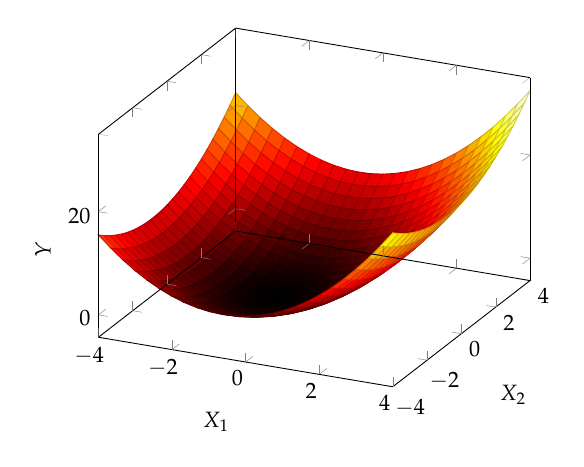
\begin{tikzpicture}[scale=0.8]
  \pgfdeclarelayer{pre main}
  \pgfsetlayers{pre main,main}
  \begin{axis}[
      xlabel=$X_1$,
      ylabel=$X_2$,
      zlabel=$Y$,
      xmin=-4, xmax=4,
      ymin=-4, ymax=4,
      domain = -4:4,
      zmax   = 35,
      colormap/hot2
    ]
    \begin{pgfonlayer}{pre main}
      \addplot3 [surf] {(2.5*x + 1.75*y + 2*x^2+y^2)/2};
    \end{pgfonlayer}
  \end{axis}
\end{tikzpicture}
\caption*{Equation: $Y = 2.5X_1 + 1.75X_2 + 2X_1^2 + X_2^2$}
\end{figure}

\end{frame}


\begin{frame}{LPR: implementation (I)}
  A window width is chosen, usually in terms of \% of data (similar to kernel smoothers).\bigskip

  Within each bin, a WLS estimation of the polynomial specification is conducted.

  \begin{equation}
    \frac{Y_i}{w_i} = \frac{a}{w_i} + b_1\frac{X_i}{w_i} + b_2\frac{X_i^2}{w_i} + \dots + b_p\frac{X_i^p}{w_i} + \frac{e_i}{w_i}
    \label{eq:eq-01}
  \end{equation}

  The $w_i$ are typically assigned with the tricube kernel used in kernel smoothing.
\end{frame}



\begin{frame}{LPR: implementation (II)}
  In a second stage, a set of robustness weights is obtained from the specification in Equation \ref{eq:eq-01}. These are then applied to the model, for another round of estimation.\bigskip

  Then we start again with the $w_i$, then with robustness weights.\bigskip

  The process stops when there is minimal change in estimates from one iteration to another.\bigskip

  The use of $w_i$ is what distinguishes \textit{lowess} from \textit{loess}.
\end{frame}



\begin{frame}{LPR for Perot vote}



\begin{figure}
  \centering
  \includegraphics[scale=0.7]{../04-graphs/04-07a}
  \caption{LPR with span of 0.30}
\end{figure}

\end{frame}



\begin{frame}{LPR for Perot vote}

\begin{figure}
  \centering
  \includegraphics[scale=0.7]{../04-graphs/04-07b}
  \caption{LPR with span of 0.45}
\end{figure}
  
\end{frame}


\begin{frame}{LPR for Perot vote}

\begin{figure}
  \centering
  \includegraphics[scale=0.7]{../04-graphs/04-07c}
  \caption{LPR with span of 0.60}
\end{figure}
  
\end{frame}



\begin{frame}{Local polynomials: choices}

  In practice, it does not matter very much whether it's \textit{loess} or \textit{lowess}, or the polynomial order ($p$).\bigskip

  The span matters:

  \begin{itemize}
  \item very low $\Rightarrow$ low bias, but high variance: ``undersmoothing'';
  \item very high $\Rightarrow$ high bias, but low variance: ``oversmoothing''.
  \end{itemize}\bigskip

  A middle ground has to be found by the researcher, but with erring on the side of ``undersmoothing'' \cite[p.~34]{keele2008}.\footnote{Same with polynomial order: better fit vs. extra parameters.}
  
\end{frame}




\subsection{Inference in LPR}

\begin{frame}{Inference}

  Since at each step a regression is run, inference based on SEs can be easily conducted.\footnote{The formulas for this are no longer nice, so I omit them here, but you can get a quick look at them in \citeA[pp.~39--41]{keele2008}}\bigskip

  This is usually displayed on the plot, in the form of confidence intervals around the line.
   
\end{frame}



\begin{frame}{Inference for Perot vote}



\begin{figure}
  \centering
  \includegraphics[scale=0.7]{../04-graphs/04-08}
  \caption{LPR with span of 0.50 and SEs}
\end{figure}
   
\end{frame}



\begin{frame}{Hypothesis testing}
  An even more powerful application is to test whether the nonparametric model fits the data better than the parametric linear one.\bigskip

  We can do this as the latter model is a restricted version of the former.

  \begin{equation}
    F = \frac{\frac{RSS_0 - RSS_1}{J}}{\frac{RSS_1}{df_{res}}}
  \end{equation}

  $df_{res} = n - p_1$, where $p_1$ is the effective number of parameters of the smoother, and $n$ is the sample size.\bigskip

  $df_{res}$ need not be an integer in the case of smoothers.
  
\end{frame}



\begin{frame}{Hypothesis testing}
  The other terms in the formula:

  \begin{itemize}
  \item $RSS_0$: residual sum of squares from restricted specification;
  \item $RSS_1$: residual sum of squares from nonparametric specification;
  \item $J = p_1 - p_0$: difference in effective number of parameters
  \end{itemize}



In this case, the F-test $=4.742065$, and $p<0.001$, suggesting that the nonparametric model fits the data better.
  
\end{frame}
  





\section{Splines}


\begin{frame}
\begin{center}
    \Huge Regression Splines
\end{center}
\end{frame}


\begin{frame}{Advantages of splines}

\noindent\begin{minipage}{0.4\textwidth}% adapt widths of minipages to your needs
\includegraphics[width=\linewidth]{../04-graphs/Spline-old-school}
\end{minipage}%
\hfill%
\begin{minipage}{0.5\textwidth}
  \begin{itemize}
  \item will provide the best mean squared error fit;
  \item a smoothing spline is designed to prevent overfitting;
  \item easier to incorporate in semiparametric models than LPR.
  \end{itemize}
\end{minipage}

\end{frame}



\begin{frame}{The use of \textit{knots}}
  Splines are essentially polynomials fitted to separate regions of the data.\bigskip

  The ``borders'' between these regions are called \textit{knots} (just values of $X$).\bigskip

  The polynomials are fit to the separate regions, and forced to meet at the \textit{knot}.

\end{frame}



\begin{frame}[fragile]{Piece-wise polynomials}



\begin{figure}
	\centering
	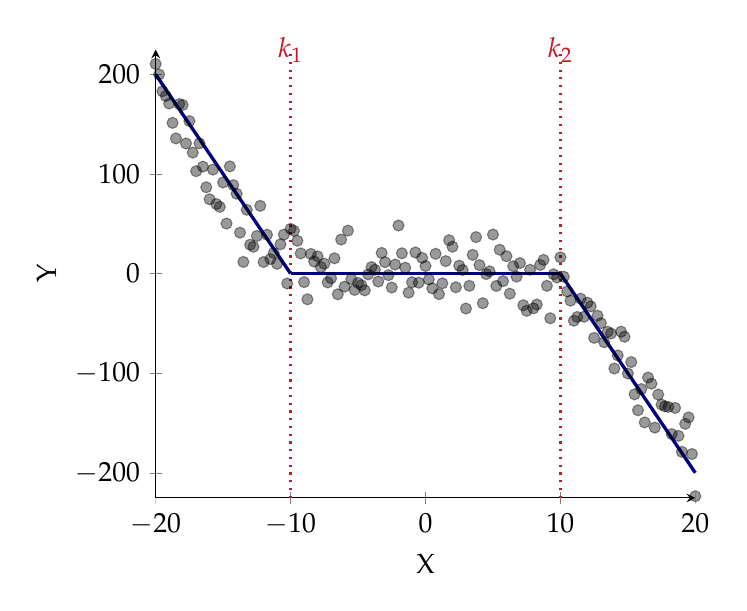
\begin{tikzpicture}
	\pgfplotstableread{
x y
-20	210.596
-19.75	200.038
-19.5	183.202
-19.25	178.385
-19	170.889
-18.75	151.492
-18.5	135.861
-18.25	170.371
-18	169.4
-17.75	130.797
-17.5	153.257
-17.25	121.634
-17	102.95
-16.75	130.941
-16.5	107.537
-16.25	86.824
-16	74.774
-15.75	104.541
-15.5	69.979
-15.25	67.178
-15	91.678
-14.75	50.355
-14.5	107.813
-14.25	88.979
-14	80.329
-13.75	41.248
-13.5	11.899
-13.25	64.245
-13	29.158
-12.75	27.049
-12.5	37.911
-12.25	68.192
-12	11.826
-11.75	39.19
-11.5	14.731
-11.25	20.888
-11	9.989
-10.75	29.612
-10.5	39.286
-10.25	-9.758
-10	45.055
-9.75	43.147
-9.5	33.117
-9.25	20.444
-9	-8.4
-8.75	-25.648
-8.5	19.903
-8.25	12.297
-8	17.516
-7.75	6.654
-7.5	10.086
-7.25	-8.703
-7	-4.461
-6.75	15.518
-6.5	-20.596
-6.25	34.348
-6	-12.95
-5.75	43.306
-5.5	-5.378
-5.25	-16.242
-5	-9.195
-4.75	-11.472
-4.5	-16.683
-4.25	-0.634
-4	6.706
-3.75	4.056
-3.5	-7.773
-3.25	20.916
-3	11.66
-2.75	-1.419
-2.5	-13.802
-2.25	9.257
-2	48.438
-1.75	20.56
-1.5	6.067
-1.25	-18.962
-1	-8.506
-0.75	21.422
-0.5	-8.989
-0.25	15.899
0	7.808
0.25	-5.713
0.5	-14.614
0.75	20.037
1	-20.471
1.25	-9.603
1.5	12.694
1.75	33.682
2	27.164
2.25	-13.512
2.5	8.13
2.75	3.789
3	-34.874
3.25	-12.091
3.5	18.957
3.75	36.795
4	8.72
4.25	-29.551
4.5	-0.377
4.75	2.486
5	39.369
5.25	-12.231
5.5	24.107
5.75	-7.403
6	17.62
6.25	-19.995
6.5	7.557
6.75	-2.881
7	10.743
7.25	-31.588
7.5	-37.184
7.75	4.028
8	-34.718
8.25	-30.894
8.5	8.832
8.75	13.918
9	-12.108
9.25	-44.639
9.5	-0.555
9.75	-3.74
10	16.498
10.25	-2.976
10.5	-17.762
10.75	-27.004
11	-47.163
11.25	-43.352
11.5	-25.046
11.75	-43.133
12	-28.993
12.25	-32.745
12.5	-64.338
12.75	-42.107
13	-49.567
13.25	-68.775
13.5	-58.202
13.75	-59.918
14	-95.139
14.25	-81.971
14.5	-58.152
14.75	-63.221
15	-100.135
15.25	-88.634
15.5	-121.016
15.75	-137.007
16	-115.73
16.25	-149.206
16.5	-104.17
16.75	-110.348
17	-154.434
17.25	-121.261
17.5	-131.357
17.75	-133.097
18	-133.658
18.25	-160.906
18.5	-134.667
18.75	-162.704
19	-178.737
19.25	-150.637
19.5	-144.18
19.75	-180.9
20	-223.297
}\loadedtable
	\begin{axis}[
	xlabel=X, % label x axis
	ylabel=Y, % label y axis
	axis lines=left, %set the position of the axes
	xmin=-20, xmax=20, % set the min and max values of the x-axis
	ymin=-225, ymax=225, % set the min and max values of the y-axis
	clip=false
	]

	\addplot [only marks, opacity=0.4] table {\loadedtable};
	\draw[dotted, thick, title] (100,0)--(100,450) node {$k_1$};
	\draw[dotted, thick, title] (300,0)--(300,450) node {$k_2$};
	\draw[very thick, NavyBlue] (0,425.0876)--(100,225.15964);
	\draw[very thick, NavyBlue] (100,225.15964)--(300,225.15964);
	\draw[very thick, NavyBlue] (300,225.15964)--(400,25.1847);
	
	\end{axis}
      \end{tikzpicture}
\caption{Very simple example, with 1st order polynomial and 2 knots}
\end{figure}

\end{frame}



\begin{frame}{Piece-wise polynomials}
The number of knots, their position, as well as the degree of the polynomial specification are chosen by the researcher.\bigskip

For most realistic problems, only 4--5 knots are really needed.\bigskip

Let's take the situation of a single knot:

\begin{equation}
Y_i = a + b_1X_i + b_2(X_i)_+ + e_i
\end{equation}
\end{frame}




\begin{frame}{Piece-wise polynomials}
  This $(X)_+$ is a new variable, which we obtain from $X$, based on its position with respect to $c_1$ (the knot position).\bigskip

  \begin{equation}
    (x_i)_+ = \begin{cases}
         x_i, & \text{for}\ x_i > c_1 \\
           0, & \text{for}\ x_i \leq c_1.      
      \end{cases}
    \end{equation}

    \begin{equation}
    Y_i = \begin{cases}
         a + b_1X_i, & \text{for}\ x_i \leq c_1 \\
         a + b_1X_i + b_2(X_i - c_1), & \text{for}\ x_i > c_1.      
      \end{cases}
    \end{equation}
  
\end{frame}



\begin{frame}{More complex forms}
  So far, I have only used linear specifications, as they make the formulas accessible.\bigskip

  However, we can easily specify quadratic and cubic specifications, in case the data patterns reveal such forms are needed.\bigskip

  \begin{itemize}
  \item knots can be added by default at the lowest and highest data points, so as to fit cubic splines in these regions as well: \textit{natural splines};
  \item piece-wise functions can be rescaled, so as to avoid collinearity between $X$ and $(X)_+$: \textit{B-splines}. 
  \end{itemize}
  
\end{frame}


\begin{frame}[fragile]{More complex forms}

\begin{figure}
	\centering
	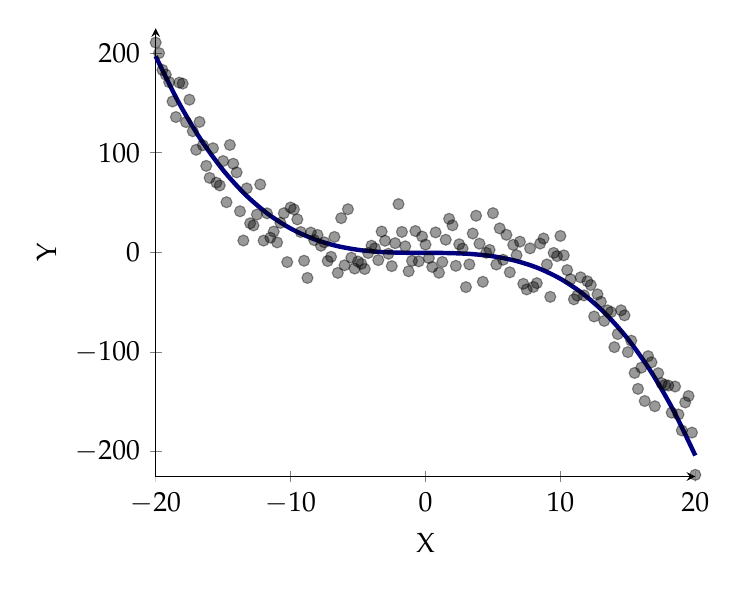
\begin{tikzpicture}
	\pgfplotstableread{
x y
-20	210.596
-19.75	200.038
-19.5	183.202
-19.25	178.385
-19	170.889
-18.75	151.492
-18.5	135.861
-18.25	170.371
-18	169.4
-17.75	130.797
-17.5	153.257
-17.25	121.634
-17	102.95
-16.75	130.941
-16.5	107.537
-16.25	86.824
-16	74.774
-15.75	104.541
-15.5	69.979
-15.25	67.178
-15	91.678
-14.75	50.355
-14.5	107.813
-14.25	88.979
-14	80.329
-13.75	41.248
-13.5	11.899
-13.25	64.245
-13	29.158
-12.75	27.049
-12.5	37.911
-12.25	68.192
-12	11.826
-11.75	39.19
-11.5	14.731
-11.25	20.888
-11	9.989
-10.75	29.612
-10.5	39.286
-10.25	-9.758
-10	45.055
-9.75	43.147
-9.5	33.117
-9.25	20.444
-9	-8.4
-8.75	-25.648
-8.5	19.903
-8.25	12.297
-8	17.516
-7.75	6.654
-7.5	10.086
-7.25	-8.703
-7	-4.461
-6.75	15.518
-6.5	-20.596
-6.25	34.348
-6	-12.95
-5.75	43.306
-5.5	-5.378
-5.25	-16.242
-5	-9.195
-4.75	-11.472
-4.5	-16.683
-4.25	-0.634
-4	6.706
-3.75	4.056
-3.5	-7.773
-3.25	20.916
-3	11.66
-2.75	-1.419
-2.5	-13.802
-2.25	9.257
-2	48.438
-1.75	20.56
-1.5	6.067
-1.25	-18.962
-1	-8.506
-0.75	21.422
-0.5	-8.989
-0.25	15.899
0	7.808
0.25	-5.713
0.5	-14.614
0.75	20.037
1	-20.471
1.25	-9.603
1.5	12.694
1.75	33.682
2	27.164
2.25	-13.512
2.5	8.13
2.75	3.789
3	-34.874
3.25	-12.091
3.5	18.957
3.75	36.795
4	8.72
4.25	-29.551
4.5	-0.377
4.75	2.486
5	39.369
5.25	-12.231
5.5	24.107
5.75	-7.403
6	17.62
6.25	-19.995
6.5	7.557
6.75	-2.881
7	10.743
7.25	-31.588
7.5	-37.184
7.75	4.028
8	-34.718
8.25	-30.894
8.5	8.832
8.75	13.918
9	-12.108
9.25	-44.639
9.5	-0.555
9.75	-3.74
10	16.498
10.25	-2.976
10.5	-17.762
10.75	-27.004
11	-47.163
11.25	-43.352
11.5	-25.046
11.75	-43.133
12	-28.993
12.25	-32.745
12.5	-64.338
12.75	-42.107
13	-49.567
13.25	-68.775
13.5	-58.202
13.75	-59.918
14	-95.139
14.25	-81.971
14.5	-58.152
14.75	-63.221
15	-100.135
15.25	-88.634
15.5	-121.016
15.75	-137.007
16	-115.73
16.25	-149.206
16.5	-104.17
16.75	-110.348
17	-154.434
17.25	-121.261
17.5	-131.357
17.75	-133.097
18	-133.658
18.25	-160.906
18.5	-134.667
18.75	-162.704
19	-178.737
19.25	-150.637
19.5	-144.18
19.75	-180.9
20	-223.297
}\loadedtable
	\begin{axis}[
	xlabel=X, % label x axis
	ylabel=Y, % label y axis
	axis lines=left, %set the position of the axes
	xmin=-20, xmax=20, % set the min and max values of the x-axis
	ymin=-225, ymax=225, % set the min and max values of the y-axis
	clip=false
	]

	\addplot [only marks, opacity=0.4] table {\loadedtable};
  \draw[domain=-20:20,smooth,variable=\x,NavyBlue, ultra thick] plot ({\x*10+200},{(-0.5 - 0.025*\x - 0.0075*\x*\x - 0.025*\x*\x*\x)+225});
	\end{axis}
	\end{tikzpicture}
\end{figure}

\end{frame}


\begin{frame}{Knot placement and \#}
  Usually placed at equal intervals in the data, e.g. quartiles or quintiles.\bigskip

  The number of knots is the more important choice---it governs how smooth the final fit will be.\bigskip

  2 methods:

  \begin{itemize}
  \item visual: start with 4 knots, and increase/decrease number if the fit is too smooth/rough;
  \item statistical: use the AIC of the fit, and select the number of knots that produces the lowest AIC.
  \end{itemize}
  
\end{frame}


\begin{frame}{Splines for Perot vote}
  


\begin{figure}
  \centering
  \includegraphics[scale=0.7]{../04-graphs/04-09}
  \caption{\textcolor{RoyalBlue}{Cubic B-spline} and \textcolor{RedOrange}{natural spline} fits}
\end{figure}

\end{frame}



\subsection{Smoothing splines}


\begin{frame}
\begin{center}
    \Huge Smoothing splines
\end{center}
\end{frame}


\begin{frame}{Penalized splines}
  One frequent accusation is that it's very easy to overfit the data with splines, as you can simply select a large number of knots.\bigskip

  Penalized (smoothing) splines are a solution to this, as they introduce a penalty for every additional parameter estimated.\footnote{In the same way that the adjusted $R^2$ includes such a penalty.}

  \begin{equation}
    SSR = \sum_{i=1}^n[Y - f(X)]^2
  \end{equation}

  In standard linear regression this $f(X)$ is the model specification.
  
\end{frame}



\begin{frame}{Penalized splines}
  For penalized splines, a modified version of $SSR$ gets minimized.

  \begin{equation}
    SSR^* = \sum_{i=1}^n[Y - f(X)]^2 + \lambda\int_{x_1}^{x_n}[f^{''}(x)]^2dx
  \end{equation}

  $f^{''}(x)$ is the second derivative to the nonlinear fit. The less smooth the curve, the higher this second derivative is.

  $\lambda$ is called the smoothing (tuning) parameter. The higher it is, the smoother the fit (but, also, more biased).
  
\end{frame}



\begin{frame}{Penalized splines}
  Because of the smoothing parameter, $\lambda$, the number of \textit{knots} does not matter that much anymore.\bigskip

  Allowing for any order of derivative, $f^{m}(x)$, produces what are called \textit{thin plate splines}. These are useful for smoothing in larger number of dimensions.\bigskip

  Constructing confidence intervals and hypothesis tests (with the $F$-test) proceeds the same as with standard splines based on piece-wise polynomials.
  
\end{frame}



\begin{frame}{Penalized splines}


  
\begin{figure}
  \centering
  \includegraphics[scale=0.7]{../04-graphs/04-10}
  \caption{Smoothing spline with 4 knots and $\lambda=0.00179$.}
\end{figure}  

\end{frame}



\begin{frame}{Penalized splines}

\begin{figure}
  \centering
  \includegraphics[scale=0.7]{../04-graphs/04-11}
  \caption{Smoothing spline with 10 knots and $\lambda=0.00179$.}
\end{figure}  
\end{frame}


% FRAME
\begin{frame}
\begin{center}
    \Huge Thank \textcolor{title}{you} for the kind attention!
\end{center}
\end{frame}

% REFERENCES %

\begin{frame}[allowframebreaks]{References}
\bibliographystyle{apacite}
\bibliography{../Bibliography}
\end{frame}

\end{document}
